\subsection{Terraform}
\begin{otherlanguage}{ngerman}
\subsubsection{Funktionsweise}
\textit{Terraform} ist eine \textit{Open-Source-Software}, welche die Vorbereitung von \textit{Cloud Servern} einfacher macht. Sie wurde von HashiCorp dazu entwickelt, Infrastrukturen vorzubereiten und zu verwalten.\footcite{introform} Mit Infrastrukturen sind hier \textit{virtuelle Maschinen} verschiedenster Anbieter gemeint.\footnote{\cite{Terraform}} Terraform hat lizenzierte Partner für die seine Dienste anwendbar sind.\footcite{TerraProviders} Durch die hohe Konnektivität dieser Software sind die Einsatzorte sehr vielseitig. Das macht die Software in der Entwicklung und im Betrieb von Unternehmen sehr attraktiv. 
\newline
\newline
Terraform ist ein Infrastructure-as-Code-Tool und wird für die Bereitstellung von physischen als auch virtuellen Servern verwendet. Das Tool arbeitet mit Konfigurationsdateien, die in der HashiCorp Configuration Language(HCL) geschrieben werden. Die genannten Dateien sind von Menschen lesbar und gewährleisten dadurch die geringe Komplexität der Sprache. Zudem ist HCL eine deklarative Sprache. Das heißt, dass der Nutzer den Wunschaufbau des Servers in der Terraform-Datei beschreibt. Die einzelnen Schritte um den gewünschten Serverzustand zu erreichen werden von Terraform übernommen. 
\newline
Die Prozesse in die die Arbeit mit Terraform unterschieden werden kann, sind in drei Schritte aufgeteilt. Der erste Schritt ist \tt write \rm. In dieser Phase wird der Code definiert. Dafür werden die benötigten Ressourcen für die jeweiligen Provider definiert. Dafür Terraform-Konfigurations-Dateien mit der Endung \tt .tf \rm verwendet. Aus diesen Dateien entnimmt Terraform beispielsweise welcher Cloud-Anbieter verwendet wird. Als Beispiel für einen Anbieter mit dem Terraform funktioniert können die Microsoft Azure-Dienste genannt werden. Zu den Providern findet sich auf der Seite von Terraform eine jeweilige Dokumentation darüber, wie die Ressourcen einzubinden sind. Der Code der Konfigurations-Dateien entscheidet darüber, wie der Server konfiguriert wird, wenn dass script ausgeführt wird. 
\newline
Wenn der Code verfasst wurde folgt der nächste Schritt im Arbeitsablauf von Terraform. Dieser ist die Planung der vorgenommenen Aktionen. Wird \tt terraform apply \rm in der Kommandozeile eingegeben so wird dieser Plan erstellt. Dieser wird im Anschluss daran ausgegeben. Um Fortzufahren muss der Plan, indem jeder Schritt aufgelistet ist, den Terraform durchführen wird, bestätigt werden. Diese einzelnen Schritte können Änderungen, Löschungen oder das Hinzufügen von Dateien sein.
\begin{figure}
    \centering
    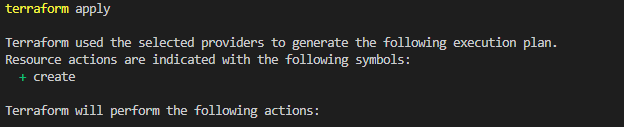
\includegraphics{LaTeX/graphic/terraformapply.png}
    \caption{Terraform - Planungsphase}
\end{figure}
%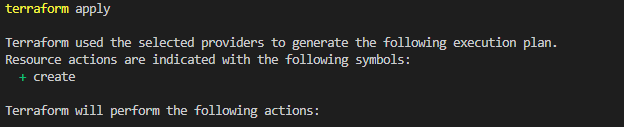
\includegraphics[]{LaTeX/graphic/terraformapply.png}
\addcontentsline{lof}{figure} {Terraform - Was macht der Befehl 'apply'}
\newpage 
Die Dritte und letzte Phase im Terraform-Workflow ist \tt apply \rm. Sie beginnt mit der Bestätigung des Plans. Ab diesem Zeitpunkt beginnt Terraform mit der Bereitstellung des Servers. Welche Systemkomponenten und Sicherheitseinstellungen dieser hat ist von den Konfigurationsdateien abhängig. 
\newpage
\subsubsection{Vorteile}
-schnell
\newline
-variabel
\newline
-nicht allzu komplex
\end{otherlanguage}